%%%%%%%%%%%%%%%%%%%%%%%%%%%%%%%%%%%%%%%%%%%%%%%%%%%%%%%%%%%%%%%%%%%%%%%%%%%%%%%%
\chapter{Обзор и анализ систем инструментирования программ}
%%%%%%%%%%%%%%%%%%%%%%%%%%%%%%%%%%%%%%%%%%%%%%%%%%%%%%%%%%%%%%%%%%%%%%%%%%%%%%%%

В данном разделе рассматривается понятие инструментирования, а также проводится сравнительный обзор некоторых существующих средств, позволяющих автоматизировать выполнение этого процесса с некоторым вовлечением пользователя.

%%%%%%%%%%%%%%%%%%%%%%%%%%%%%%%%%%%%%%%%%%%%%%%%%%%%%%%%%%%%%%%%%%%%%%%%%%%%%%%%
\section{Понятие инструментирования}
%%%%%%%%%%%%%%%%%%%%%%%%%%%%%%%%%%%%%%%%%%%%%%%%%%%%%%%%%%%%%%%%%%%%%%%%%%%%%%%%

Под \underline{инструментированием} обычно понимают возможность отслеживания или установления количественных параметров программного продукта, а также возможность диагностировать ошибки и записывать информацию для отслеживания причин их возникновения посредством встраивания дополнительного (инструментирующего) кода в исследуемое ПО \cite{lomakina2016testirovanie}.
\nomenclature[0]{ПО}{программное обеспечение.}

Наиболее распространенными областями применения инструментирования являются \cite{instrumentiruieto}:

\begin{itemize}[noitemsep]
  \item трассировка;
  \item отладка;
  \item регистрация событий;
  \item подмена кода;
  \item счетчики производительности и др.
\end{itemize}

В зависимости от специфики используемого ЯП, среды его выполнения и доступности исходного текста инструментируемого ПО возможны три основных варианта инструментирования:
\nomenclature[0]{ЯП}{язык программирования.}

\begin{itemize}[noitemsep]
  \item инструментирование на уровне исходного текста;
  \item инструментирование бинарного кода;
  \begin{itemize}[noitemsep]
    \item инструментирование промежуточного кода;
    \item инструментирование машинного кода.
  \end{itemize}
\end{itemize}

%%%%%%%%%%%%%%%%%%%%%%%%%%%%%%%%%%%%%%%%%%%%%%%%%%%%%%%%%%%%%%%%%%%%%%%%%%%%%%%%
\subsection{Пример задачи инструментирования}
%%%%%%%%%%%%%%%%%%%%%%%%%%%%%%%%%%%%%%%%%%%%%%%%%%%%%%%%%%%%%%%%%%%%%%%%%%%%%%%%
Ниже рассмотрен упрощенный пример задачи, которая часто решается путем инструментирования требуемого фрагмента или полного исходного кода программного продукта.

Пусть дан следующий фрагмент исходного текста (функция) на некотором языке программирования (в данном случае -- JavaScript) \cite{instrumentiruieto}:
\begin{lstlisting}[frame=single, language=Java]
function foo(a) {
    if (a > 5) {
        return 1;
    } else {
        return 2;
    }
}
\end{lstlisting}

Задача: необходимо выяснить, сколько раз и какие строки этого фрагмента (тела функции) выполняются при проведении тестирования некоторым тестом $T$ (содержимое и результаты работы теста не рассматриваются; подразумевается, что тест сравнивает результат работы вызова этой функции с некоторыми аргументами с каким-то, заранее заданным, фиксированным значением).

Решение: разместим вызовы некоторой функции \lstinline{__visit(x)}, где x -- номер строки или порядковый номер отслеживаемой точки, перед каждой интересующей строкой, число исполнений которой необходимо определить.

Результатом такого преобразования будет являться следующий исходный текст:
\begin{lstlisting}[frame=single, language=Java]
function foo(a) {
    __visit(1);
    if (a > 5) {
        __visit(2);
        return 1;
    } else {
        __visit(3);
        return 2;
    }
}
\end{lstlisting}

В приведенном выше примере аргументами функции \lstinline{__visit(x)} является порядковые номера частей, количество раз выполнения которых необходимо найти.
Сама функция \lstinline{__visit(x)} в данном примере будет иметь следующий вид \cite{instrumentiruieto}:
\begin{lstlisting}[frame=single, language=Java]
// количество нулей соответствует общему количеству точек в исходном тексте, число исполнений которых необходимо измерить
var __count = [0, 0, 0, ...];

window.__visit = function(idx) {
    __count[idx - 1]++;
};
\end{lstlisting}

В данном случае массив \lstinline{__count} по окончании работы теста $T$ будет содержать число вызовов функции \lstinline{__visit(x)}, и соответственно, количество раз, сколько были выполнены интересующие строки исходного фрагмента кода.

В табл.~\ref{table:insrtExampleResults} приведен пример определения целевого показателя (число исполнений каждой строки исходного фрагмента).
\begin{table}[H]
  \captionsetup{skip=5pt}
  \caption{Пример сопоставления результатов.}
  \label{table:insrtExampleResults}
  \centering
  \begin{tabular}{|c|c|c|c|}
    \hline
    \# п.п., i  & Исходный участок            & \lstinline!__count[i]!  & Число исполнений  \\ \hline
    1           & \lstinline!if (a > 5)!      & 10                      & 10                \\ \hline
    2           & \lstinline!{ return 1; }!   & 7                       & 7                 \\ \hline
    3           & \lstinline!{ return 2; }!   & 3                       & 3                 \\ \hline
  \end{tabular}
\end{table}

Как видно из результатов, примененный способ ценой дополнительных расходов памяти на хранение массива \lstinline{__count} решает поставленную задачу.

Схожим способом можно решить задачу определения времени исполнения каждого блока (и отдельно взятой строки) в исходном тексте, промежуточном представлении или даже машинном коде инструментируемого ПО, вместе с множеством других задач, которые требуют встраивание небольших фрагментов кода в какие-то заранее определенные области исходного кода.

Однако, для масштабного и частого применения данного метода необходимы средства, позволяющие в автоматическом режиме произвести подобные трансформации с исходным текстом, промежуточным представлением или машинным представлением, в зависимости от специфики ЯП и доступности исходного текста.

%%%%%%%%%%%%%%%%%%%%%%%%%%%%%%%%%%%%%%%%%%%%%%%%%%%%%%%%%%%%%%%%%%%%%%%%%%%%%%%%
\subsection{Достоинства и недостатки различных вариантов инструментирования}
%%%%%%%%%%%%%%%%%%%%%%%%%%%%%%%%%%%%%%%%%%%%%%%%%%%%%%%%%%%%%%%%%%%%%%%%%%%%%%%%
Инструментирование на уровне исходного текста подразумевает вставку инструментального кода до компиляции (сборки) ПО.

Рассмотрим некоторые достоинства инструментирования исходного текста по сравнению с модификацией на уровне машинного кода \cite{lomakina2016testirovanie}:
\begin{itemize}[noitemsep]
  \item большая производительность, поскольку инструментальный код подвергается оптимизации вместе с кодом анализируемой программы;
  \item возможность отслеживания работы с высокоуровневыми объектами языка программирования (например, отслеживание состояния объектов в объектно-ориентированных языках).
\end{itemize}

Однако, данный метод инструментирования обладает рядом недостатков, ограничивающих его применимость \cite{lomakina2016testirovanie}:
\begin{itemize}[noitemsep]
  \item для выполнения анализа требуется сборка специального исполняемого образа, что неприменимо на поздних стадиях жизненного цикла программного продукта;
  \item сложность обработки взаимодействия инструментируемого и неинструментируемого кода (например, в случае использования разделяемых библиотек);
  \item сложность реализации инструментирования -- необходимость синтаксического анализа исходного текста с учетом индивидуальных особенностей компиляторов, нестандартных расширений языка и т.п.
\end{itemize}

Инструментирование на уровне бинарного кода подразумевает вставку инструментального кода во время компиляции (на одном из этапов) или после получения финальных артефактов сборки (исполняемых файлов).

Инструментирование на уровне бинарного кода обладает следующими преимуществами \cite{lomakina2016testirovanie}:
\begin{itemize}[noitemsep]
  \item Большая гибкость -- независимость от языка программирования и отсутствие требования наличия исходных текстов. Возможно применение к итоговым образам на поздних этапах жизненного цикла продукта.
  \item Анализ с точностью до инструкции и до каждого доступа к памяти.
  \item Анализ программы после применения всех оптимизаций компилятора, позволяющий обнаруживать ошибки в итоговых исполняемых образах, включая ошибки компилятора.
  \item Простота использования -- не требуется специальная сборка ПО, достаточен запуск под подходящей виртуальной машиной.
  \item Программная система обрабатывается в целом -- инструментированию подвергается как сам тестируемый модуль, так и все используемые им стандартные средства, что позволяет учесть преобразования данных, осуществляемые в стандартных подпрограммах.
\end{itemize}

Недостатки инструментирования бинарного кода \cite{lomakina2016testirovanie}:
\begin{itemize}[noitemsep]
  \item меньшая производительность по сравнению с методами, работающими на уровне исходных текстов;
  \item сложность сопоставления машинных инструкций и операторов исходного языка программирования (для этого используется отладочная информация, однако это вызывает трудности в случае применения флагов оптимизации при сборке исходного ПО).
\end{itemize}

%%%%%%%%%%%%%%%%%%%%%%%%%%%%%%%%%%%%%%%%%%%%%%%%%%%%%%%%%%%%%%%%%%%%%%%%%%%%%%%%
\section{Обзор существующих средств инструментирования}
%%%%%%%%%%%%%%%%%%%%%%%%%%%%%%%%%%%%%%%%%%%%%%%%%%%%%%%%%%%%%%%%%%%%%%%%%%%%%%%%

Далее будут рассмотрены с позиции различных критериев некоторые существующие автоматизированные системы инструментирования, позволяющие произвести инструментирование исходных текстов программного обеспечения.

%%%%%%%%%%%%%%%%%%%%%%
\subsection{Критерии обзора}
%%%%%%%%%%%%%%%%%%%%%%

Критерии обзора будут основываться на ситуации, когда пользователю требуется выполнять обработку исходных текстов программ на новом языке программирования или нескольких существующих.
При этом обработка заключается во встраивании дополнительного кода, позволяющего производить измерение каких-либо специфических параметров (или в более общем случае -- выполнение инструментирования) в соответствии с решаемой пользователем задачей.
С учетом этого, выделим следующие критерии сравнения систем инструментирования:

\begin{itemize}[noitemsep]
  \item Поддерживаемые языки программирования.
  \item Источник средств анализа исходных текстов.
  \item Исполнение -- иснтрументирующее приложение выполнено как часть большей системы или в виде отдельной программы.
  \item Возможности пользователя самостоятельно расширять спектр поддерживаемых ЯП.
\end{itemize}

%%%%%%%%%%%%%%%%%%%%%%
\subsection{GCC Gcov}
%%%%%%%%%%%%%%%%%%%%%%
Свободно распространяемая утилита gcov, которая предоставляет информацию о том, сколько раз исполнился во время работы программы каждый участок исходного текста.

Утилита создает файл формата <<.gcda>> с анализом покрытия кода для программ, инструментированных с помощью опций <<\lstinline{-fprofile-arcs -ftest-coverage}>> компиляторов в составе GNU Compiller Collection (GCC), что является основой её функционирования \cite{reviewGCCGcov}. Первая опция приводит к сохранению статистики исполнения каждой строки исходного файла, а вторая -- статистики ветвлений.
\nomenclature{GCC}{GNU Compiller Collection -- набор компиляторов для различных языков программирования, разработанный в рамках проекта GNU.}

Набор компиляторов GCC поддерживает несколько языков программирования приложений, включая Ada, C, C++, Fortran, Objective-C, Objective-C++, Go и D \cite{reviewGCC}. Таким образом, утилита GCC Gcov способна выполнять инструментирование исходных текстов программ, созданных с использованием языков Ada, C, C++, Fortran, Objective-C, Objective-C++, Go, D, при условии использовании последних версий компиляторов из набора GCC.

Важным ограничением возможностей утилиты является требование об отключении опций оптимизации при сборке инструментируемого ПО, что иначе приведет к некорректным, неполным или неожиданным результатам \cite{reviewGCCGcov}.

После запуска инструментированной программы будет создано несколько файлов с расширениями <<.bb>>, <<.bbg>>, <<.da>>, которые в последствии будут анализироваться gcov. Утилита принимает в качестве аргумента командной строки имена файлов с исходными текстами и производит аннотированный листинг: перед каждой строкой исходного кода указывается количество её исполнений, строки, которые не исполнялись, помечаются префиксом <<\#\#\#\#\#>> \cite{reviewGCCGcov}.

%%%%%%%%%%%%%%%%%%%%%%
\subsection{Testwell CTC++ Preprocessor}
%%%%%%%%%%%%%%%%%%%%%%
Testwell CTC++ -- это коммерческая система инструментального покрытия кода и динамического анализа для кода C и C++. С некоторыми дополнительными компонентами CTC ++ можно использовать также для C\#, Java и Objective-C. Кроме того, CTC ++ может использоваться для анализа кода на встраиваемых машинах, в том числе с ограничениями по ресурсам (малое количество памяти, отсутствие ОС и др.). Система обеспечивает покрытие кода для отдельных строк, выражений, функций, ветвлений \cite{reviewCTC}.

Утилита CTC++ Preprocessor (ctc) используется для инструментирования и компиляции представляющих интерес исходных файлов C или C++ и для связывания инструментированной программы с библиотекой времени выполнения CTC++. На этом этапе уилита ctc использует файл символов <<MON.sym>>, где сохраняются имена инструментированных файлов и их содержимое.

Система CTC++ используется вместо стандартного компилятора, предоставляя собственный для используемого ЯП, что позволяет гибко встраивать инструментальный код \cite{reviewCTC}.

%%%%%%%%%%%%%%%%%%%%%%
\subsection{BullseyeCoverage}
%%%%%%%%%%%%%%%%%%%%%%
BullseyeCoverage -- это коммерческий анализатор покрытия кода для программ, созданных с использованием языков программирования C и C++, который позволяет собрать статистическую информацию о полноте тестирования программного кода. Анализ покрытия кода бывает полезен при проведении модульного, интеграционного и финального тестирования программного продукта.

Препроцессор системы BullseyeCoverage использует возможности компилятора Microsoft C++ для сборки инструментированного кода, что позволяет выполнять инструментирование под разными процессорами и платформами, которые поддерживаются этим компилятором \cite{reviewBullseyeCoverage}.

%%%%%%%%%%%%%%%%%%%%%%
\subsection{Google Web Tracing Framework}
%%%%%%%%%%%%%%%%%%%%%%
Web Tracing Framework (WTF) -- это свободно распространяемый набор библиотек, инструментов и сценариев, предназначенных для веб-разработчиков, пытающихся писать большие, чувствительные к производительности приложения JavaScript. Он предназначен для использования вместе со встроенными инструментами разработки браузеров \cite{reviewWTF}. 

WTF предоставляет возможности по перехвату событий, инструментированию кода, трассировки и отображения собранной статистики посредством встроенных возможностей среды исполнения JavaScript, в частности, браузера Google Chrome \cite{reviewWTF}. Инструментирование осуществляется вызовом специализированных функций этой библиотеки.

%%%%%%%%%%%%%%%%%%%%%%
\subsection{Froglogic Squish Coco CoverageScanner}
%%%%%%%%%%%%%%%%%%%%%%
Squish Coco -- это многоязычный (Tcl, QML, C\#, C/C++) коммерческий инструмент для автоматической оценки покрытия исходного кода, используемый для измерения охвата тестами сценариями блоков кода, ветвлений и условных выражений.

На рис.~\ref{fig:froglogic_coco} приведена обобщенная схема процесса инструментирования и отображения результатов.

\begin{figure}[!h]
	\centering
	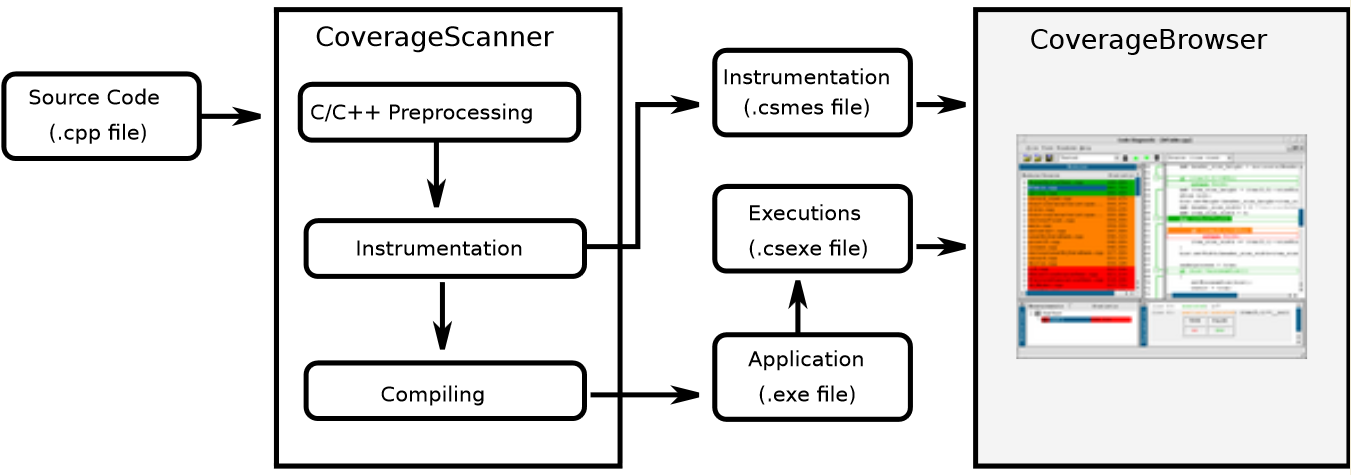
\includegraphics[width=4.2in]{froglogic_coco}
	\caption{Cхема работы Coco CoverageScanner.}
	\label{fig:froglogic_coco}
\end{figure}

Утилита CoverageScanner осуществляет анализ, предобработку и инструментирование временной копии исходного текста, который впоследствии перенаправляется выбранному компилятору. Гибкость создается благодаря подмене с помощью скриптов (командных сценариев) вызовов компиляторов и средств сборки так, чтобы одним (первым) из этапов сборки оказалась утилита CoverageScanner \cite{reviewFrog}.

%%%%%%%%%%%%%%%%%%%%%%%%%%%%%%%%%%%%%%%%%%%%%%%%%%%%%%%%%%%%%%%%%%%%%%%%%%%%%%%%
\section{Итоги}
%%%%%%%%%%%%%%%%%%%%%%%%%%%%%%%%%%%%%%%%%%%%%%%%%%%%%%%%%%%%%%%%%%%%%%%%%%%%%%%%

В табл.~\ref{table:reviewResultsCompare} собраны основные сведения о рассмотренных системах инструментирования в соответствии с обозначенными критериями обзора.
\begin{table}[htbp]
  \centering
  \captionsetup{skip=5pt}
  \caption{Основные характеристики систем инструментирования.}
  \resizebox{0.99\textwidth}{!}{\begin{minipage}{\textheight}
    \label{table:reviewResultsCompare}
    \begin{tabular}{|l|c|c|c|c|}
      \hline
      Название системы                                                         & Поддерживаемые языки                                                            & \vtop{\hbox{\strut Средства }\hbox{\strut анализа}}  & Исполнение                                                  & \vtop{\hbox{\strut Расширение }\hbox{\strut поддержки ЯП}} \\ \hline
      GCC Gcov                                                                 & \vtop{\hbox{\strut Ada, C/C++, Fortran, Go, }\hbox{\strut Objective-C/C++, D}}  & внешние                                              & \vtop{\hbox{\strut встроено в }\hbox{\strut компилятор }}   & \vtop{\hbox{\strut ответвление }\hbox{\strut проекта }} \\ \hline
      \vtop{\hbox{\strut Testwell CTC++ }\hbox{\strut Preprocessor}}           & \vtop{\hbox{\strut C/C++, C\#, }\hbox{\strut Java, Objective-C }}               & встроенные                                           & \vtop{\hbox{\strut собственный }\hbox{\strut компилятор }}  & отсутствует \\ \hline
      BullseyeCoverage                                                         & C/C++                                                                           & встроенные                                           & препроцессор                                                & отсутствует \\ \hline
      \vtop{\hbox{\strut Google Web Tracing }\hbox{\strut Framework}}          & Javascript                                                                      & встроенные                                           & препроцессор                                                & \vtop{\hbox{\strut ответвление }\hbox{\strut проекта }} \\ \hline
      \vtop{\hbox{\strut Froglogic Squish Coco }\hbox{\strut CoverageScanner}} & Tcl, QML, C\#, C/C++                                                            & встроенные                                           & препроцессор                                                & отсутствует \\ \hline
    \end{tabular}
  \end{minipage}}
\end{table}

Из представленных результатов видно отсутствие решений с требуемой функциональностью:
каждый из перечисленных проектов работает только с очень небольшым множеством языков программирования и для организации работы с новым (для системы) языком для всех проектов, за исключением коммерческих проектов, необходимо создание и поддержка заинтересованным пользователем ответвления от основной кодовой базы, что связано с большими временными и трудовыми расходами.
Ввиду того, что проекты Testwell CTC++, BullseyeCoverage и Froglogic Squish Coco предоставляется на коммерческих условиях использования, внесением дополнительных возможностей, в том числе увеличение числа поддерживаемых языков программирования, занимается исключительно соответствующая компания-разработчик.

Исходя из этого можно сделать заключение о необходимости создания  автоматизированной системы инструментирования, которая была бы способна работать с несколькими языками программирования или имела возможность подстраиваться под требуемый ЯП при некоторой помощи со стороны пользователя такой системы.

%%%%%%%%%%%%%%%%%%%%%%%%%%%%%%%%%%%%%%%%%%%%%%%%%%%%%%%%%%%%%%%%%%%%%%%%%%%%%%%%
\section{Выводы}
%%%%%%%%%%%%%%%%%%%%%%%%%%%%%%%%%%%%%%%%%%%%%%%%%%%%%%%%%%%%%%%%%%%%%%%%%%%%%%%%

В данном разделе было проведено ознакомление с понятием инструментирования, приведены достоинства и недостатки различных видов инструментирования, рассмотрен простейший пример процесса инструментирования программного обеспечения и выполнен краткий обзор некоторых существующих средств, позволяющих выполнять этот процесс автоматически для программных продуктов, созданных с использованием различных языков программирования.

По результатам обзора было сделано заключение о необходимости создания автоматизированной системы инструментирования программ, которая имела бы возможность работать с текстами программ на различных языках программирования.
